\chapter{Exponential Function}%

\section{Definition of an exponential function}%

\dfn{}{
    Let $a>0$ and $x\in\mathbb{R}$. The function $f(x)=a^x$ is called the exponential function with base $a$.
}

Based on the above definition we have:
\begin{enumerate}
    \item $f(x)=2^x$ is the exponential function with base $2$.
    \item $f(x)=e^x$ is the exponential function with base $e$.
\end{enumerate}

\dfn{}{
    Consider the exponential function with the form $f(x)=b*a^{x-h}+k$ with $f:\mathbb{R}\to\mathbb{R}$; 
    $f$ is an exponential function if and only if $a\in]0,1[$ or $a\in]1,\infty[$.
}

Some exponential functions with the form $f(x)=b*a^{x-h}+k$ are:
\begin{itemize}
    \item $f(x)=2^{x-1}+1$
    \item $f(x)=\frac{1}{2}^{x-1}-8$
\end{itemize}

\section{Properties}%

\thm{}{
    If the base is negative, the function is not defined for all real numbers.\\
    Let's consider a function $f(x)=(-3)^x$.

    \paragraph{At $x=\frac{1}{2}$.}
    \begin{equation}
        \begin{aligned*}
            f\left(\frac{1}{2}\right) &= (-3)^{\frac{1}{2}} \\
                                      &= \sqrt{-3} \\
                                      &= \pm i\sqrt{3}
        \end{aligned*}
    \end{equation}

    Hence, the base of an exponential function cannot be negative.
}

\thm{}{
    If the function is in the form $f(x)=a^x$, then the function is not transformed, 
    and doesn't have a vertical or horizontal shift.\\
    This also means that the function doesn't have an intersection with the $x$-axis 
    and the asymptoten is $y=0$.
}

\thm{}{
    When $x=0$ or $x=1$ the function is constant. It means that isn't an exponential function at these $x$ values.
    For this is why the domain of the exponential function is defined like this: $D_f:]0,1[\cup]1,\infty[$
    \begin{itemize}
        \item If the function base is $1$, then the function is constant and $y=1$.\\
        \item If the function base is $0$, then the function is constant and equal to $0$.
    \end{itemize}
}

\section{Graphs}%

Consider the graph of the function $f(x)=a^x$, $f:\mathbb{R}\to\mathbb{R}^+$.
\begin{itemize}
    \item The figure \ref{fig:exp-case-1} shows the graph of the function, where $a$ is defined in the interval $]0,1[$.
    \item The figure \ref{fig:exp-case-2} shows the graph of the function, where $a$ is defined in the interval $]1,\infty[$.
\end{itemize}

\begin{figure}[htpb]
    \centering
    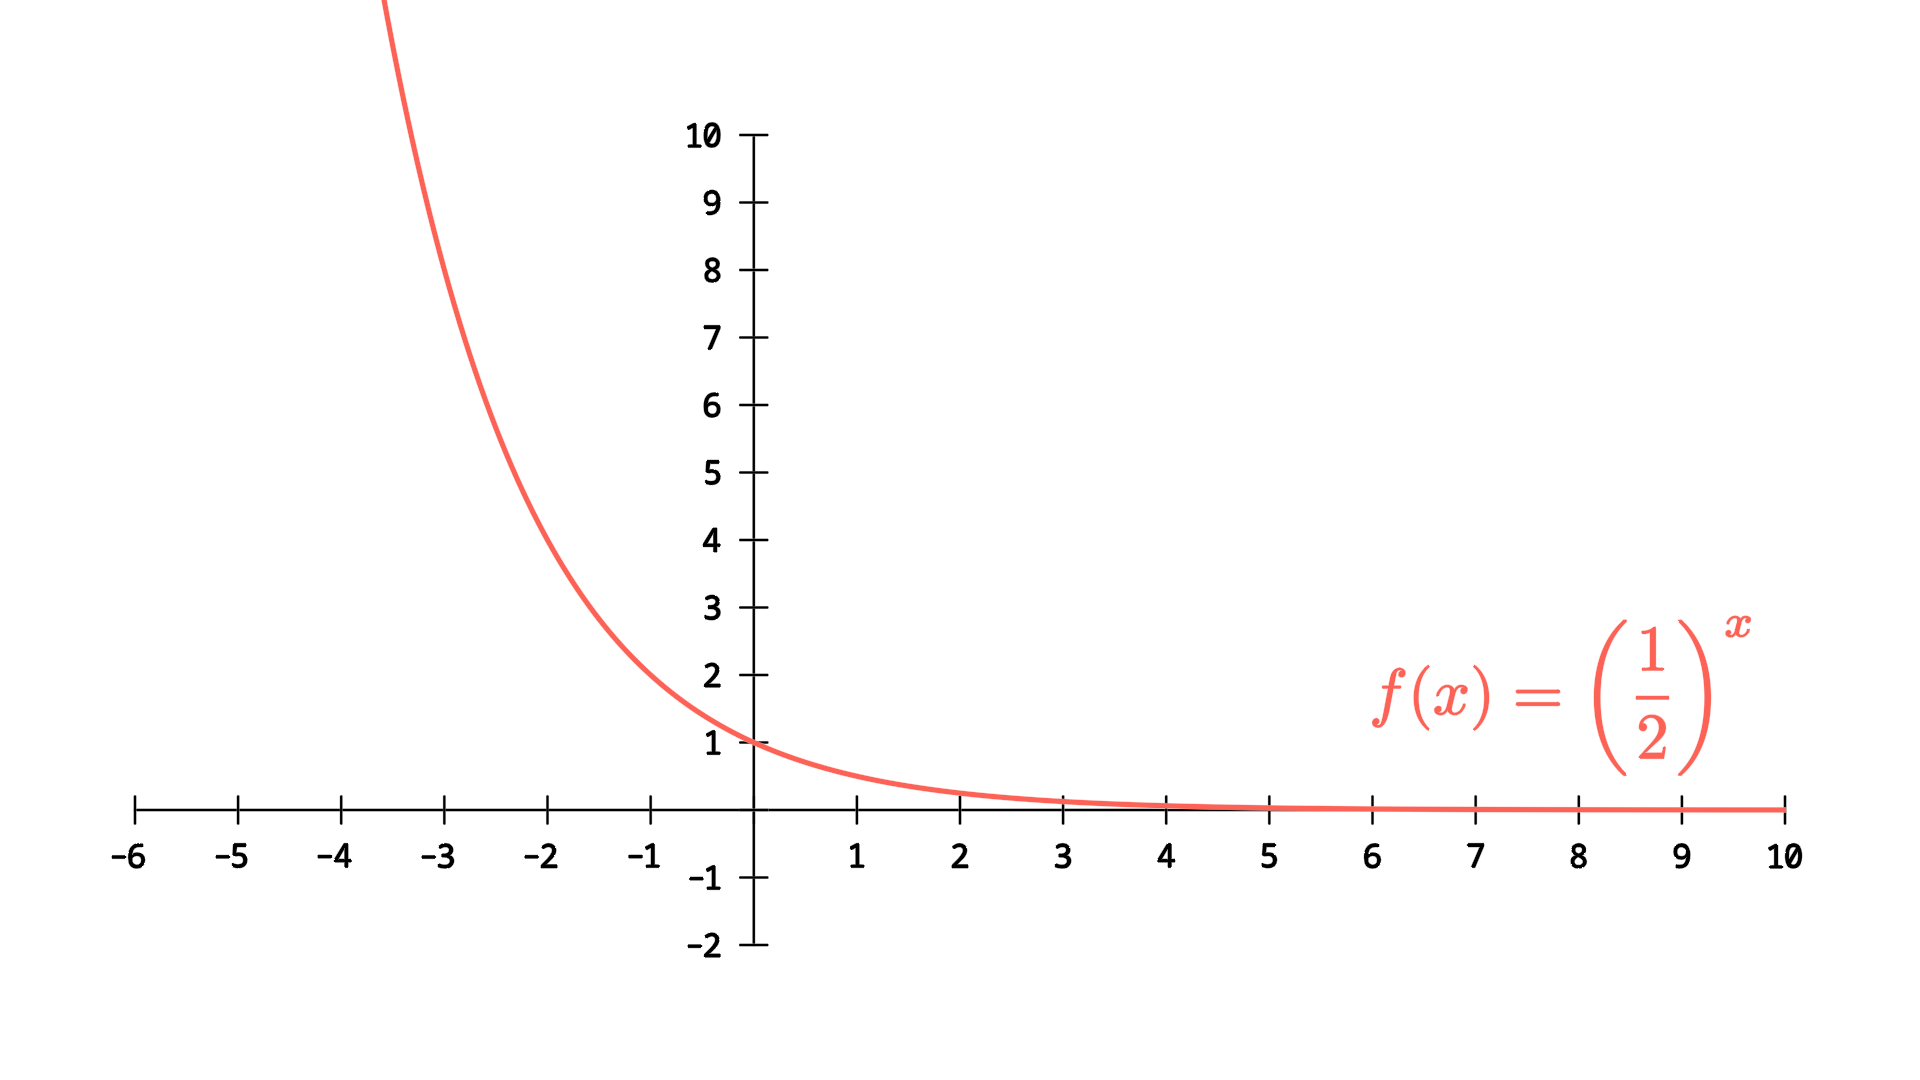
\includegraphics[width=0.8\textwidth]{images/exp-case-1.png}
    \caption{Case in which $0<a<1$.}
    \label{fig:exp-case-1}
\end{figure}

\begin{figure}[htpb]
    \centering
    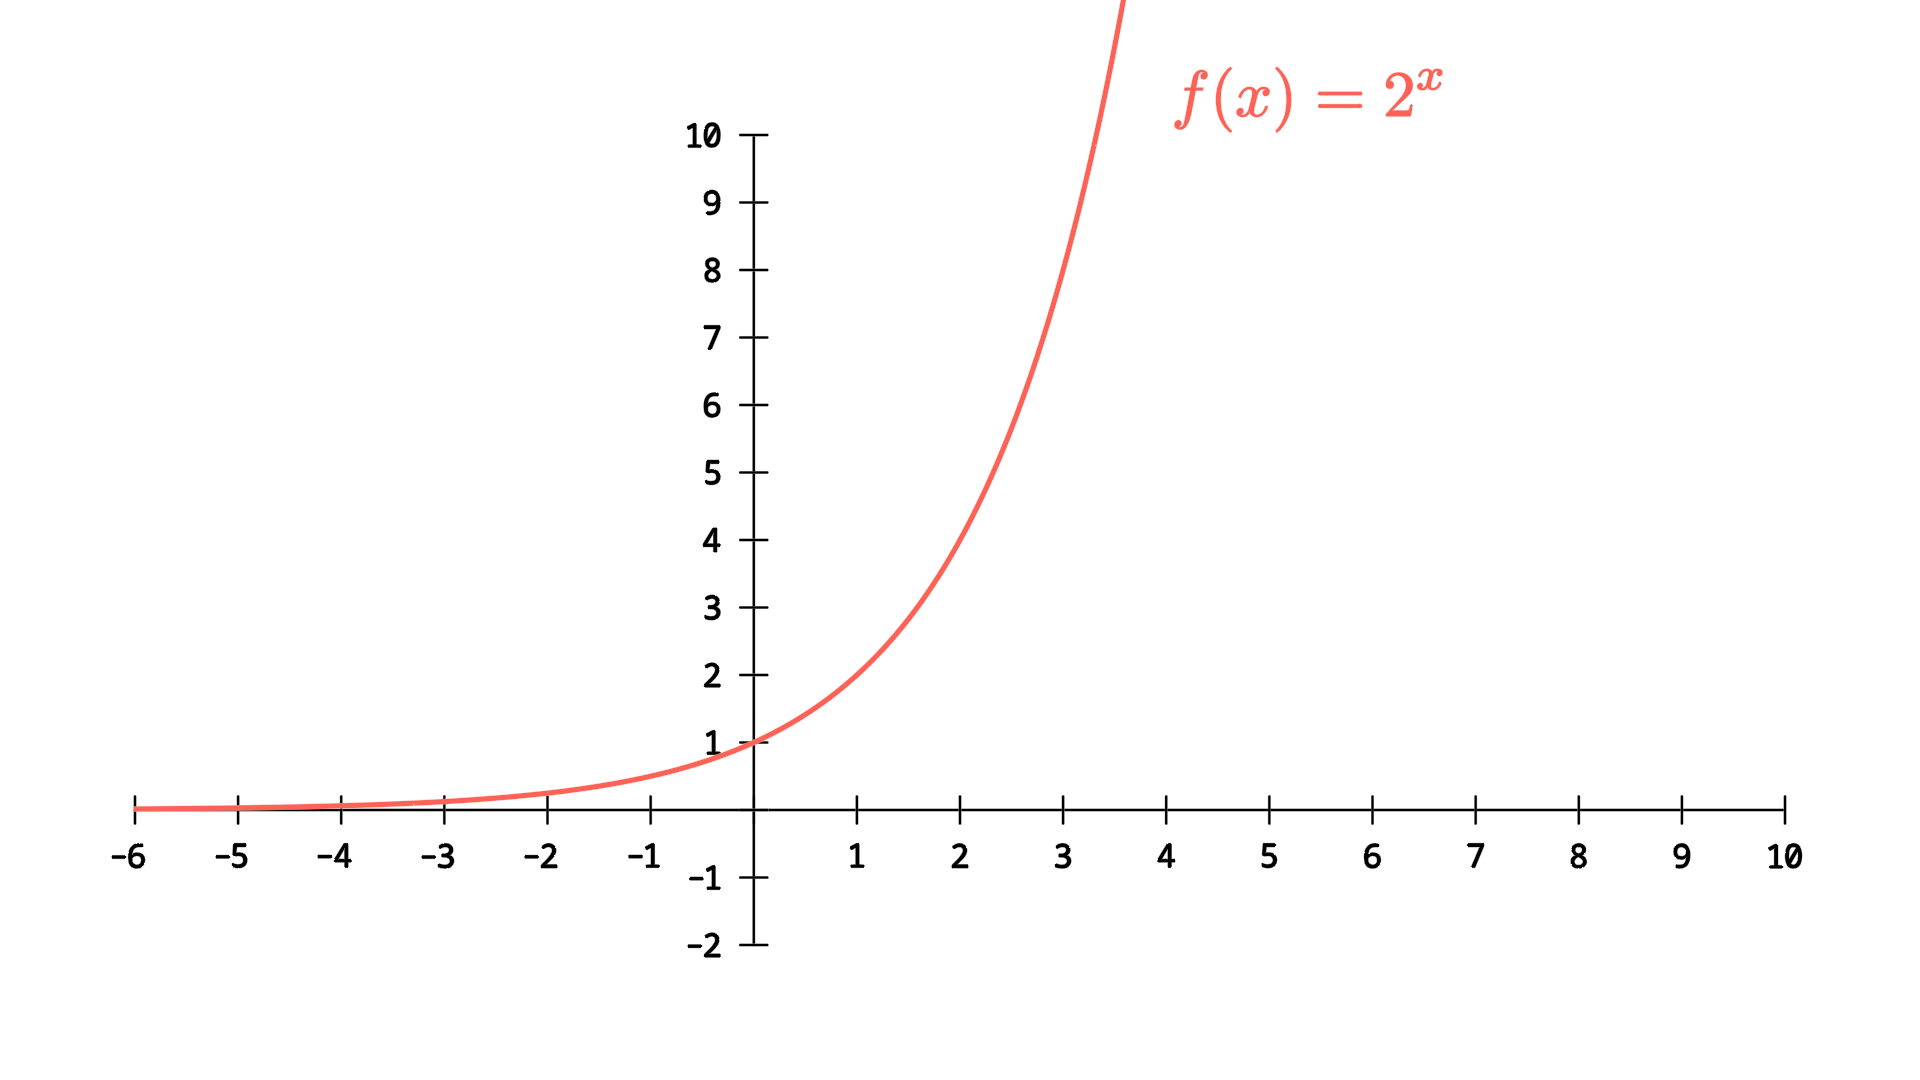
\includegraphics[width=0.8\textwidth]{images/exp-case-2.png}
    \caption{Case in which $a>1$.}
    \label{fig:exp-case-2}
\end{figure}

\section{Intercepts and asymptotes}%

\thm{}{
\item The function $f(x)=a^x$ has no intercepts with the $x$-axis and the asymptoten is $y=0$.
    % TODO: Check the x intercepts.
\item The function $f(x)=b*a^{x-h}+k$ has an asymptoten in $y=k$, and if $k$ is negative the function has an intersection with the $x$-axis.
}

% \pf{Asymptoten in $y=k$ for $f(x)=b*a^{a-h}+k$}{
% \[
%     \lim_{x\to\infty}f(x)=\lim_{x\to\infty}b*a^{x-h}+k=k
% \]
% }

\begin{figure}[htpb]
    \centering
    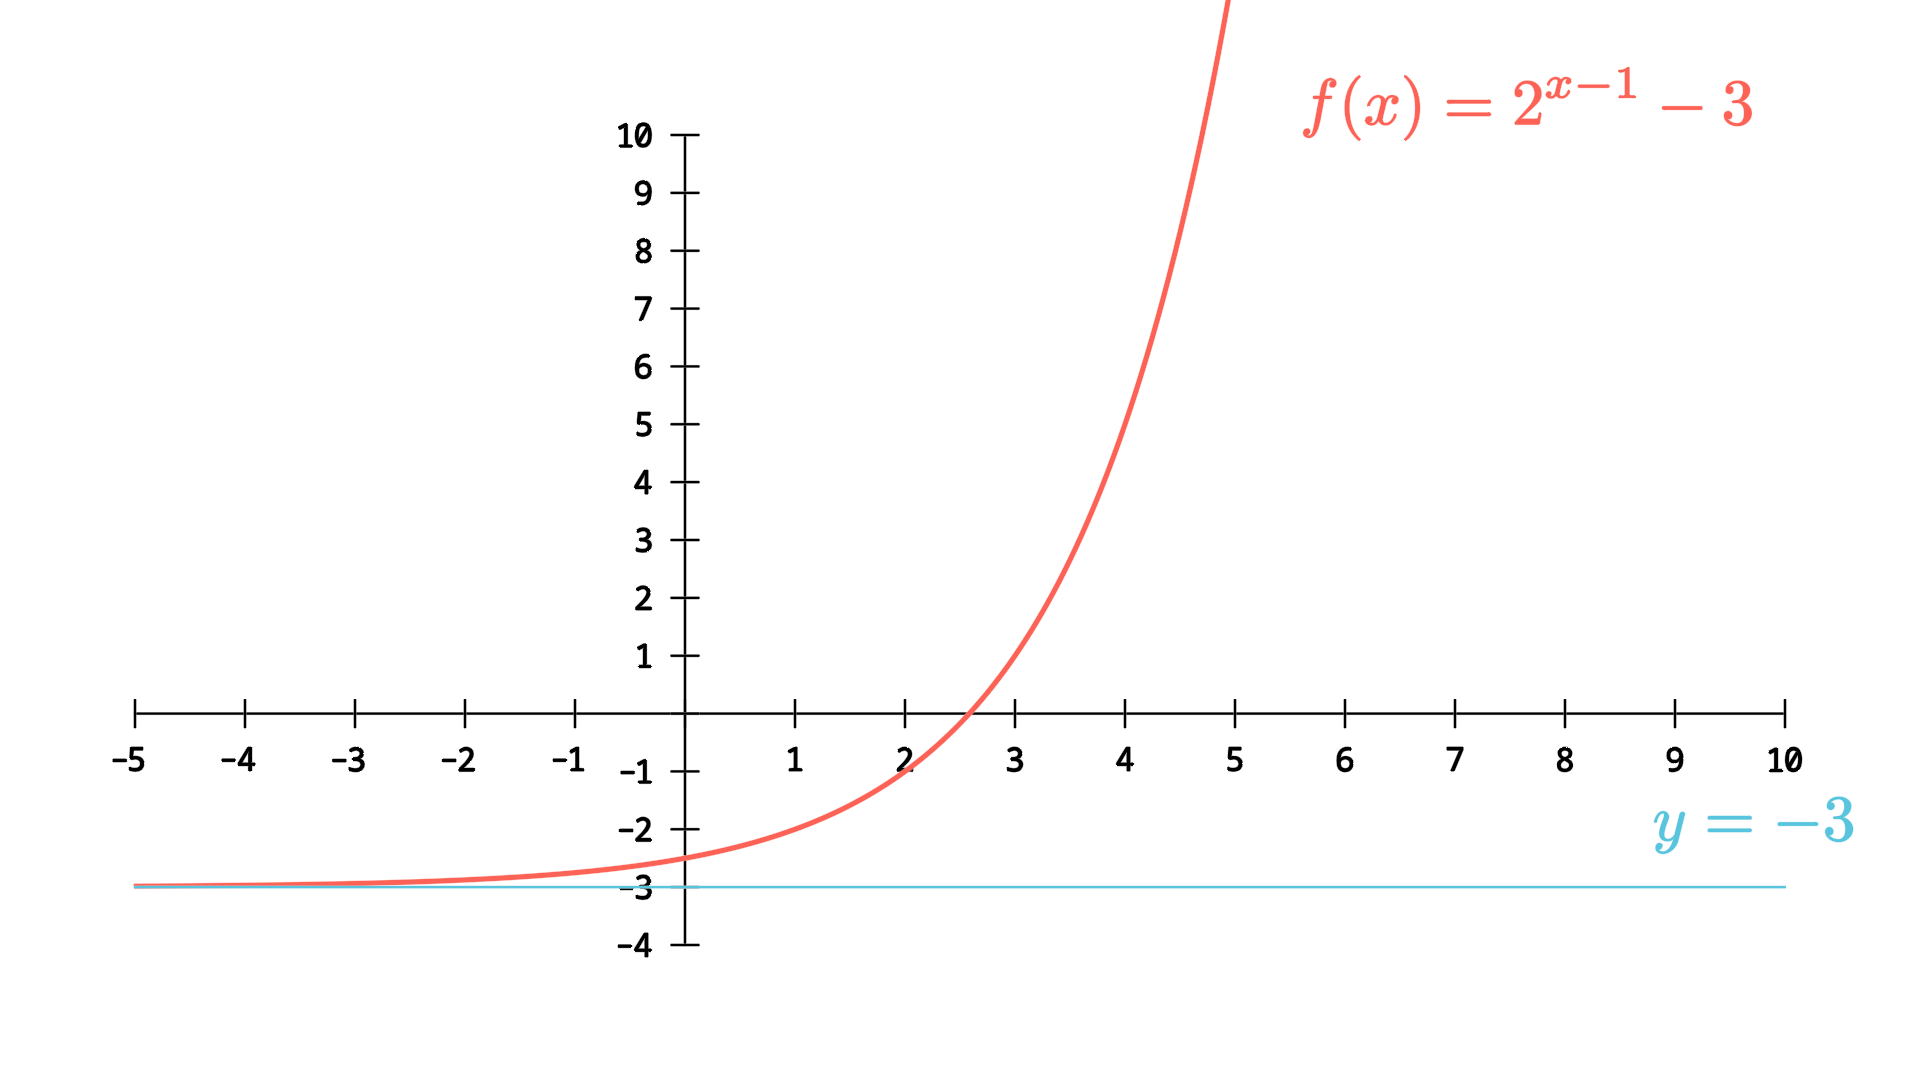
\includegraphics[width=0.8\textwidth]{images/exp-case-3.png}
    \caption{Asymptote in $y=-3$ for $f(x)=2^{x-1}-3$.}
    \label{fig:exp-asymptote}
\end{figure}

\section{Solved exercises}%
